\documentclass[10pt]{article}

\usepackage[utf8]{inputenc}
\usepackage{floatrow}

\usepackage{algorithm}
\usepackage{algorithmic}
\usepackage[T1]{fontenc}
\usepackage{enumitem}
\usepackage{hyperref}
\usepackage{graphicx}
\usepackage{color}
\usepackage{listings}
\usepackage{wrapfig}
\usepackage{amsfonts}
\usepackage{amsmath}
\usepackage{mathtools}
\usepackage[hmargin=1.25in,vmargin=1.25in]{geometry}

%title setup
\title{Projet informatique: Honshu (Lot X)}
\author{
			Romain PEREIRA\\
			Douha OURIMI\\
			Afizullah RAHMANY\\
			Guangyue CHEN
}
\date{XX/XX/XXXX}

% table of contents setup
\renewcommand{\contentsname}{Sommaire}
\usepackage{etoolbox}
\patchcmd{\thebibliography}{\section*{\refname}}{}{}{}

\hypersetup{
    colorlinks,
    citecolor=black,
    filecolor=black,
    linkcolor=blue,
    urlcolor=red
}
			
\begin{document}
	\maketitle
	\tableofcontents
	
	\newpage
	\section*{Préambule}
		Ce projet est réalisé dans le cadre de nos études à l'ENSIIE.
		L'objectif est de prendre en main des outils de 'programmation agile',
		en developpant un jeu de carte: le Honshu.
	\newline
	\begin{figure}[H]
		\begin{center}
			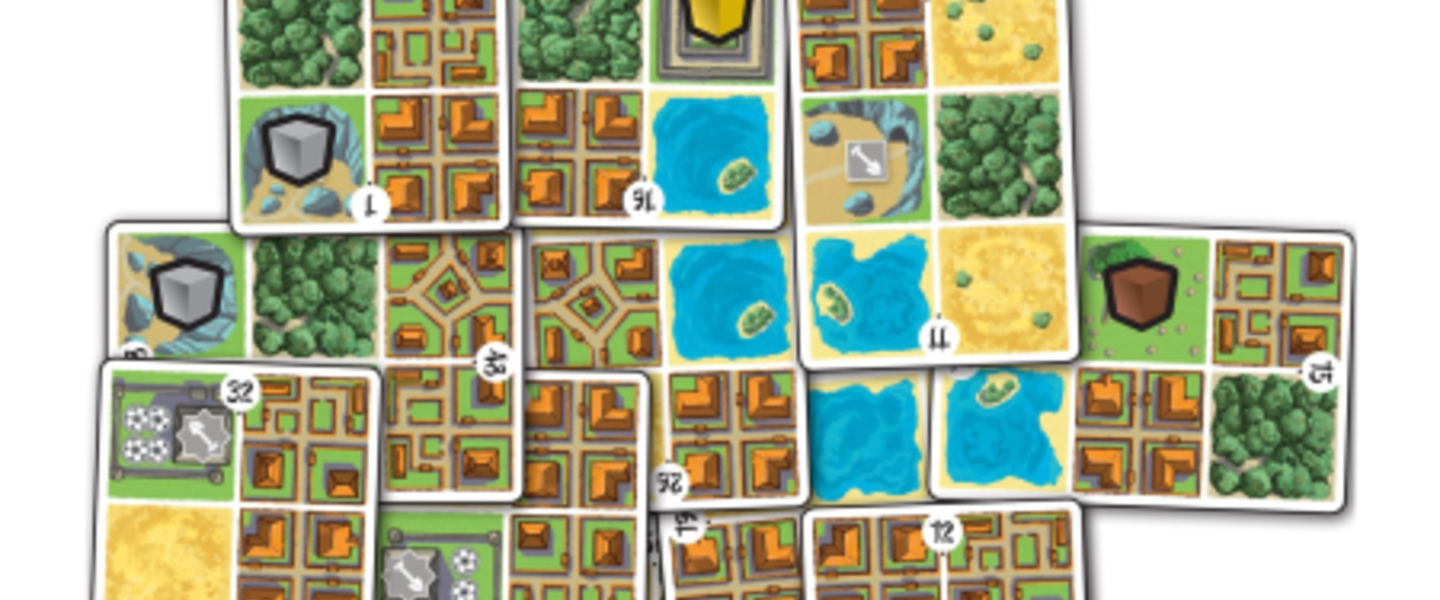
\includegraphics[height=6cm,keepaspectratio]{../images/honshu.png}
		\end{center}
		\caption{\textit{Plateau de jeu}}
		\label{honshu_introduction}
	\end{figure}

	\section{Introduction}
		Paphius quin etiam et Cornelius senatores, ambo venenorum artibus pravis se polluisse
		confessi, eodem pronuntiante Maximino sunt interfecti. pari sorte etiam procurator monetae
		extinctus est. Sericum enim et Asbolium supra dictos, quoniam cum hortaretur passim nominare,
		quos vellent, adiecta religione firmarat, nullum igni vel ferro se puniri iussurum, plumbi validis...
	\newpage
	\section{Rapport lot X}
		\subsection{XX/XX/XX}
		\subsection{XX/XX/XX}
		\subsection{XX/XX/XX}
		
	\section{Conclusion}

	\newpage
	\section{Références}
		\begin{thebibliography}{}
		\end{thebibliography}

\end{document}
